      
               
                \begin{ledgroupsized}[r]{120mm}
                \footnotesize 
                \pstart                
                \noindent\textbf{\"{U}berlieferung:}   
                \pend
                \end{ledgroupsized}
            
              
                            \begin{ledgroupsized}[r]{114mm}
                            \footnotesize 
                            \pstart \parindent -6mm
                            \makebox[6mm][l]{\textit{L}}Konzept: LH XXXVII 2 Bl. 99\textendash100. 1 Bog. 2\textsuperscript{o}. 3 S. zweispaltig. Linke Spalte fortlaufender Text, rechte Spalte Korrekturen. Auf Bl. 99 r\textsuperscript{o} in der Mitte rechts die Zeichnung \textit{[Fig. 1]}, darunter eine umfangreiche Erg\"{a}nzung, die etwa die H\"{a}lfte der Spalte ausf\"{u}llt. Auf Bl. 99 v\textsuperscript{o} rechts die Zeichnungen \textit{[Fig. 2]} und \textit{[Fig. 3]}. Bl. 100 r\textsuperscript{o} linke Spalte 1/3 beschrieben, R\"{u}ckseite leer.\\Cc 2, Nr. 492 B \pend
                            \end{ledgroupsized}
                \vspace*{8mm}
                \pstart 
                \normalsize
              \centering [99 r\textsuperscript{o}] Demonstratio Nova\\ LEGUM REFRACTIONIS,\protect\index{Sachverzeichnis}{lex!refractionis}\\ quae in lumine\protect\index{Sachverzeichnis}{lumen} observantur. \pend \vspace{1.0ex}\pstart  Mirum semper omnibus visum est, Radios Lucis\protect\index{Sachverzeichnis}{radius!lucis} ex corpore raro in densius intrantes refringi ad perpendicularem, contra ex denso in rarum exeuntes refringi a perpendiculari. Contrarium enim evenire debere videbatur, quia radius\protect\index{Sachverzeichnis}{radius!refractus} ad perpendicularem refractus medium citius fortiusque penetrat, ac profundius intrat: at medium densius ab eadem vi tardius debiliusque penetrari debere, ac radium proinde versus superficiem potius repelli, quam versus fundum refringi, rationis erat. Idque Cartesius\protect\index{Namensregister}{\textso{Descartes} (Cartesius, des Cartes, Cartes.), Ren\'{e} 1596\textendash 1650} quoque agnovit, sed rationem cur in lumine\protect\index{Sachverzeichnis}{lumen} contrarium \edtext{eveniat, eam}{\lemma{eveniat,}\Afootnote{ \textit{ (1) }\ hanc \textit{ (2) }\ eam \textit{ L}}} reddidit, quae hactenus quod sciam paucissimis, si eos adimas, qui in verba Magistri jurare parati sunt, satisfecit. Rariora scilicet ait a lumine\protect\index{Sachverzeichnis}{lumen} transiri difficilius, densiora facilius; quemadmodum globus facilius in marmore duro, polito, quam rugoso tapete \edtext{decurrat.}{\lemma{decurrat.}\Bfootnote{\textsc{R. Descartes, }\cite{00038}\textit{La dioptrique}, Leiden 1637, S.~20f. (\textit{DO} VI, S.~103).}} \edtext{Sed quam precaria quantisque difficultatibus obsita sit haec Hypothesis quam aliena similitudine confirmata dudum a multis observatum est.}{\lemma{decurrat.}\Afootnote{ \textit{ (1) }\ Sed \textit{(a)}\ quam obscura \textit{(b)}\ quam obnoxia difficultatibus \textit{(c)}\ quis concedat \textit{(aa)}\ omne rar \textit{(bb)}\ quantum unum quodque corpus est, rarius tanto esse villo. \textit{ (2) }\ Sed \textit{(a)}\ quantis difficultati \textit{(b)}\ quam [...] Hypothesis \textbar\ quam aliena similitudine \textit{ (1)}\ adhibita \textit{ (2)}\ confirmata; dudum \textit{ erg.}\ \textbar\  a multis \textit{(aa)}\ expositum est \textit{(aaa)}\ vero \textit{(bbb)}\ et ausim dicere vix \textit{(bb)}\ observatum est. \textit{ L}}} \pend \pstart  Cum ergo \edtext{}{\lemma{}\Afootnote{ergo \textbar\ nuper \textit{ gestr.}\ \textbar\ in \textit{ L}}}in Rationem quandam claram, nec quicquam nisi de quo constet assumentem, \edtext{incidissem mihi eam videari judiciis eruditorum exponere}{\lemma{assumentem,}\Afootnote{ \textit{ (1) }\ incidere, eam exponere \textit{ (2) }\ incidissem [...] exponere \textit{ L}}} volui.
                 \begin{wrapfigure}{l}{0.4\textwidth}
                 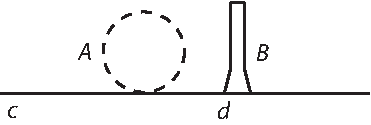
\includegraphics[width=0.4\textwidth]{images/LH37_2_99r}
                 \\\centering\textit{[Fig. 1]}
                 \end{wrapfigure}
              \edtext{Distinguendum scilicet putavi inter conatum\protect\index{Sachverzeichnis}{conatus!simplex} simplicem, et continue reparatum. Conatus simplex est; quem corpus \textit{A} exercet in obstaculum \textit{B}. Si enim obstaculum \textit{B} tantae minimum resistentiae esse supponatur, quanta est vis conatus corporis \textit{A} in obstaculum \textit{B} statim consumetur. At si loco corporis \textit{A} impingere ponatur flumen \textit{cd} in obstaculum sive aggerem \textit{B} patet ictum fluctus primi ab aliis continue insequentibus renovari, tandemque aggerem perrumpi, majore longe impetu ac fragore, quam ad primum ictum cessisset. Ajo igitur fluminis quoque ictum esse continue reparatum, ac proinde in magis obstantia fortiorem.}{\lemma{}\Afootnote{Distinguendum scilicet putavi inter conatum\protect\index{Sachverzeichnis}{conatus!simplex}  \textit{ (1) }\ simplicem \textit{ (2) }\ simplicem  \textbar\ cessantem \textit{ gestr.}\ \textbar\  , et [...] \textit{A} \textit{(a)}\ (quod Elasticum non esse supponatur, \textit{(b)}\ exercet in obstaculum \textit{B}. Si enim obstaculum  \textit{(aa)}\ ejus ictui resistat \textit{(bb)}\ primo resistere potest, \textit{(cc)}\ ei resistat, conatus \textit{(dd)}\ \textit{B} [...] vis \textit{(aaa)}\ impactus  \textit{(bbb)}\ impingentis A \textit{(ccc)}\ conatus [...] si \textit{(aaaa)}\ in obstaculum \textit{B} \textit{(bbbb)}\ loco [...] ictum \textit{(aaaaa)}\ fluminis primum \textit{(bbbbb)}\ fluctus [...] fortiorem. \textit{ erg.} \textit{ L}}} \pend \pstart Sunt autem propositiones meae ita conceptae. (1) \edtext{Conatus simplex ex \edlabel{mediostart}medio}{\lemma{(1)}\Afootnote{ \textit{ (1) }\ Motus ex med \textit{ (2) }\ Conatus simplex ex medio \textit{ L}}} \edtext{magis resistente in minus resistens oblique \edlabel{medioend}transiens}{{\xxref{mediostart}{medioend}}\lemma{medio}\Afootnote{ \textit{ (1) }\ rariore in densius transiens \textit{ (2) }\ magis [...] transiens \textit{ L}}} refringitur \edlabel{48perpendicularistart}\edtext{[a perpendiculari]}{\lemma{}\Afootnote{ad perpendicularem \textit{\ L \"{a}ndert Hrsg.}}}; \edtext{si contra ex minus resistente in magis resistens intret\edlabel{48perpendiculariend}}{{\xxref{48perpendicularistart}{48perpendiculariend}}\lemma{[perpendiculari];}\Afootnote{ \textit{ (1) }\ (2) Conatus simplex ex medio densiore in rarius transiens \textit{ (2) }\ si [...] intret \textit{ L}}} refringitur ad perpendicularem: (2) \edtext{Si obstaculo medii aucto nisus}{\lemma{(2)}\Afootnote{ \textit{ (1) }\ Nisus\protect\index{Sachverzeichnis}{nisus|textit} qui obstaculo objecto augetur \textit{ (2) }\ Si obstaculo medii aucto nisus \textit{ L}}} \edtext{quoque eo ipso fortius insurgit, ultra obstaculi renisum}{\lemma{nisus}\Afootnote{ \textit{ (1) }\ magis augetur quam obstaculum \textit{ (2) }\ quoque [...] renisum \textit{ L}}}, conatus\protect\index{Sachverzeichnis}{conatus} in medium densius \edtext{magis resistens}{\lemma{}\Afootnote{magis resistens \textit{ erg.} \textit{ L}}} ingressus refringetur ad perpendicularem. Contra si obstaculo medii diminuto, nisus quoque diminuitur infra obstaculi renisum conatus in medium \edtext{minus resistens egressus, refringetur}{\lemma{medium}\Afootnote{ \textit{ (1) }\ minus egressus \textit{ (2) }\ minus resistens egressus, refringetur \textit{ L}}} a perpendiculari. (3) Omnis nisus\protect\index{Sachverzeichnis}{nisus} continue reparatus \edtext{obstaculo objecto augetur tandem}{\lemma{reparatus}\Afootnote{ \textit{ (1) }\ magis augetur quam obstaculum \textit{ (2) }\ obstaculo objecto \textit{(a)}\ magis tand \textit{(b)}\  augetur tandem \textit{ L}}} ultra obstaculi renisum. \edtext{Idemque obstaculo tantundem diminuto quantum auctum erat redit in statum priorem}{\lemma{}\Afootnote{Idemque [...] priorem. \textit{ erg.} \textit{ L}}}. (4) Nisus\protect\index{Sachverzeichnis}{nisus} Luminis\protect\index{Sachverzeichnis}{lumen} est continue reparatus. (5) Hinc concluditur Lumen in medium densius ingressum refringi ad perpendicularem, in medium rarius egressum refringi a \edlabel{99vstart}perpendiculari.\pend  